\documentclass[aspectratio=169, 10pt]{beamer} % Formato panoramico 16:9 (standard moderno)

% --- Pacchetti Consigliati ---
\usepackage[T1]{fontenc}
\usepackage[italian]{babel}
\usepackage{graphicx}
\usepackage{subcaption}
\usepackage{booktabs} % Consigliato per tabelle professionali e pulite
\usepackage{multicol}

% --- Configurazione Tema Unipd ---
% Indica a LaTeX dove trovare le immagini
\graphicspath{{./}} 

% Carica il tema dal file beamerthemeUnipd.sty
% Opzioni:
% - pageofpages=di : cambia la dicitura nel conteggio pagine in basso
% - logo=unipd_logo_dipartimento.png : aggiunge un secondo logo alla prima pagina
% Se lo vuoi spostare un po' più a destra e in basso
\usetheme[
    pageofpages=di,
    % Regolazione logo slide interne:
    logoxshift=3mm,       % Sposta a dx (+) o sx (-) nelle slide interne
    logoyshift=0mm        % Sposta in alto (+) o in basso (-) nelle slide interne    
]{Unipd}

% --- Metadati ---
\title[Potenziale interatomico tramite machine-learning]{Messa a punto di un potenziale interatomico per la simulazione della tantala amorfa tramite machine-learning}
\subtitle{}
\author[Alberto Stocco]{Relatore: Prof. Paolo Umari \and Laureando: Alberto Stocco}
\date{Anno Accademico 2025/2026}

\begin{document}

% Pagina del Titolo ----------------------------------------------------------------------------------------------------------------
\begin{frame}[plain, noframenumbering]
    \titlepage    
\end{frame}

% Indice
%\begin{frame}{Indice}
%    \begin{multicols}{2}
%        \tableofcontents
%    \end{multicols}    
%\end{frame}

\begin{frame}{Indice}
    \begin{columns}[t]
        \begin{column}{0.48\textwidth}
            \tableofcontents[sections={1-2}]
        \end{column}
        \begin{column}{0.48\textwidth}
            \tableofcontents[sections={3-4}]
        \end{column}
    \end{columns}
\end{frame}


% --- INIZIO PRESENTAZIONE --- ----------------------------------------------------------------------------------------------------

\section{Struttura di lavoro}
\begin{frame}{Struttura di lavoro}
    \centering
    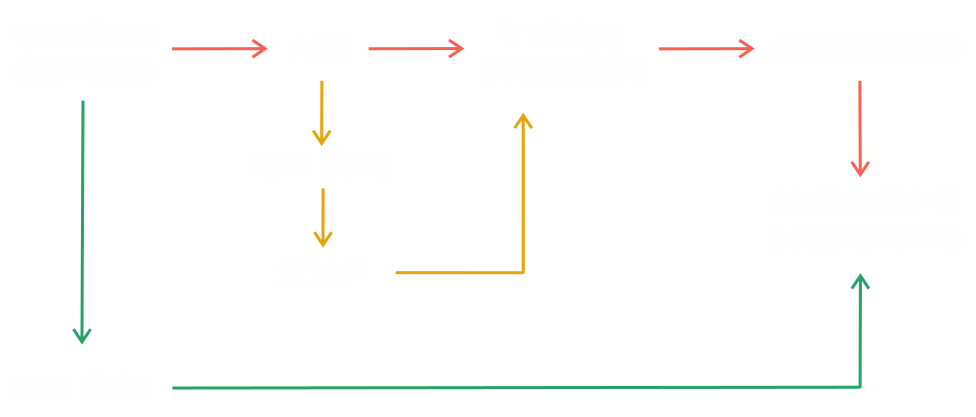
\includegraphics[scale=1.5]{invnobg/schema-lavoro - Selection.png}
\end{frame}


\subsection{SOAP} %----------------------------------------------------------------------------------------------------------------------------


\begin{frame}{SOAP}
    \begin{columns}[c]        
        % Colonna Sinistra: Testo
        \begin{column}{0.48\textwidth}
        
        -----
        
        \end{column}
        % Colonna Destra: Due immagini incolonnate
        \begin{column}{0.48\textwidth}
        
            \centering
            %\includegraphics[height=0.32\paperheight, keepaspectratio]{images/.png}
            
            \vspace{0.4cm} % Spazio verticale tra le due immagini
            
            %\includegraphics[height=0.32\paperheight, keepaspectratio]{images/.png}
            
        \end{column}
    \end{columns}
\end{frame}


\subsection{Addestramento GAP} %----------------------------------------------------------------------------------------------------------------------------


\begin{frame}{GAP}
    \begin{columns}[c]        
        % Colonna Sinistra: Testo
        \begin{column}{0.48\textwidth}
        
        -----
        
        \end{column}
        % Colonna Destra: Due immagini incolonnate
        \begin{column}{0.48\textwidth}
        
            \centering
            %\includegraphics[height=0.32\paperheight, keepaspectratio]{images/.png}
            
            \vspace{0.4cm} % Spazio verticale tra le due immagini
            
            %\includegraphics[height=0.32\paperheight, keepaspectratio]{images/.png}
            
        \end{column}
    \end{columns}
\end{frame}

\begin{frame}{GPR}
    \begin{columns}[c]        
        % Colonna Sinistra: Testo
        \begin{column}{0.48\textwidth}
        
        -----
        
        \end{column}
        % Colonna Destra: Due immagini incolonnate
        \begin{column}{0.48\textwidth}
        
            \centering
            %\includegraphics[height=0.32\paperheight, keepaspectratio]{images/.png}
            
            \vspace{0.4cm} % Spazio verticale tra le due immagini
            
            %\includegraphics[height=0.32\paperheight, keepaspectratio]{images/.png}
            
        \end{column}
    \end{columns}
\end{frame}


\subsection{Simulazione} %-------------------------------------------------------------------------------------------------------------------


\begin{frame}{Simulazione NVE}
    \begin{columns}[c]        
        % Colonna Sinistra: Testo
        \begin{column}{0.48\textwidth}
        
        -----
        
        \end{column}
        % Colonna Destra: Due immagini incolonnate
        \begin{column}{0.48\textwidth}
        
            \centering
            %\includegraphics[height=0.32\paperheight, keepaspectratio]{images/.png}
            
            \vspace{0.4cm} % Spazio verticale tra le due immagini
            
            %\includegraphics[height=0.32\paperheight, keepaspectratio]{images/.png}
            
        \end{column}
    \end{columns}
\end{frame}

\begin{frame}{ZBL}
    \begin{columns}[c]        
        % Colonna Sinistra: Testo
        \begin{column}{0.48\textwidth}
        
        -----
        
        \end{column}
        % Colonna Destra: Due immagini incolonnate
        \begin{column}{0.48\textwidth}
        
            \centering
            %\includegraphics[height=0.32\paperheight, keepaspectratio]{images/.png}
            
            \vspace{0.4cm} % Spazio verticale tra le due immagini
            
            %\includegraphics[height=0.32\paperheight, keepaspectratio]{images/.png}
            
        \end{column}
    \end{columns}
\end{frame}

\begin{frame}{Simulazione con algoritmo di Metropolis}
    \begin{columns}[c]        
        % Colonna Sinistra: Testo
        \begin{column}{0.48\textwidth}
        
        -----
        
        \end{column}
        % Colonna Destra: Due immagini incolonnate
        \begin{column}{0.48\textwidth}
        
            \centering
            %\includegraphics[height=0.32\paperheight, keepaspectratio]{images/.png}
            
            \vspace{0.4cm} % Spazio verticale tra le due immagini
            
            %\includegraphics[height=0.32\paperheight, keepaspectratio]{images/.png}
            
        \end{column}
    \end{columns}
\end{frame}

\section{Python}
\begin{frame}{Titolo della Slide}
    \begin{columns}[c]        
        % Colonna Sinistra: Testo
        \begin{column}{0.48\textwidth}
        
        to remove
        
        \end{column}
        % Colonna Destra: Due immagini incolonnate
        \begin{column}{0.48\textwidth}
        
            \centering
            %\includegraphics[height=0.32\paperheight, keepaspectratio]{images/.png}
            
            \vspace{0.4cm} % Spazio verticale tra le due immagini
            
            %\includegraphics[height=0.32\paperheight, keepaspectratio]{images/.png}
            
        \end{column}
    \end{columns}
\end{frame}


\section{Test sul dataset di QE}

\begin{frame}{Dataset A}
    \begin{columns}[c]        
        % Colonna Sinistra: Testo
        \begin{column}{0.48\textwidth}
        
        -----
        
        \end{column}
        % Colonna Destra: Due immagini incolonnate
        \begin{column}{0.48\textwidth}
        
            \centering
            
\includegraphics[scale=0.3]{./invnobg/cristallo-from-ase-frame-0-dataset-a.png}
            
        \end{column}
    \end{columns}
\end{frame}


\subsection{Energie e forze} %---------------------------------------------------------------------------------------------------------------------------


\begin{frame}{Verifica delle energie e delle forze}
    \begin{columns}[c]        
        % Colonna Sinistra: Testo
        \begin{column}{0.46\textwidth}
 
            \centering
            
            Training set 
            \vspace{6pt}
            
            
\includegraphics[scale=0.20]{./invnobg/parity_plot_gap_vs_qe-traindata.png}
            \vspace{20pt}
            
\includegraphics[scale=0.16]{./invnobg/parity_plot_forze-traindata.png}
        
        \end{column}
        % Colonna Destra: Due immagini incolonnate
        \begin{column}{0.46\textwidth}
            
            \centering
            
            Test set
            \vspace{6pt}
            
            
\includegraphics[scale=0.20]{./invnobg/parity_plot_gap_vs_qe-testdata.png}
            \vspace{20pt}
            
\includegraphics[scale=0.16]{./invnobg/parity_plot_forze-testdata.png}
            
        \end{column}
    \end{columns}
\end{frame}




\section{Simulazione}

\subsection{NVE} %----------------------------------------------------------------------------------------------------------------------------


\begin{frame}{Simulazione NVE}
    \begin{columns}[c]        
        % Colonna Sinistra: Testo
        \begin{column}{0.48\textwidth}
        
        -----
        
        \end{column}
        % Colonna Destra: Due immagini incolonnate
        \begin{column}{0.48\textwidth}
        
            \centering
            %\includegraphics[height=0.32\paperheight, keepaspectratio]{images/.png}
            
            \vspace{0.4cm} % Spazio verticale tra le due immagini
            
            %\includegraphics[height=0.32\paperheight, keepaspectratio]{images/.png}
            
        \end{column}
    \end{columns}
\end{frame}


\subsection{NVE: Analisi} %-------------------------------------------------------------------------------------------------------------------


\begin{frame}{Simulazione NVE: analisi}
    \begin{columns}[c]        
        % Colonna Sinistra: Testo
        \begin{column}{0.48\textwidth}
        
        -----
        
        \end{column}
        % Colonna Destra: Due immagini incolonnate
        \begin{column}{0.48\textwidth}
        
            \centering
            %\includegraphics[height=0.32\paperheight, keepaspectratio]{images/.png}
            
            \vspace{0.4cm} % Spazio verticale tra le due immagini
            
            %\includegraphics[height=0.32\paperheight, keepaspectratio]{images/.png}
            
        \end{column}
    \end{columns}
\end{frame}


\subsection{ZBL} %--------------------------------------------------------------------------------------------------------------------------


\begin{frame}{ZBL: risultati}
    \begin{columns}[c]        
        % Colonna Sinistra: Testo
        \begin{column}{0.48\textwidth}
        
        -----
        
        \end{column}
        % Colonna Destra: Due immagini incolonnate
        \begin{column}{0.48\textwidth}
        
            \centering
            %\includegraphics[height=0.32\paperheight, keepaspectratio]{images/.png}
            
            \vspace{0.4cm} % Spazio verticale tra le due immagini
            
            %\includegraphics[height=0.32\paperheight, keepaspectratio]{images/.png}
            
        \end{column}
    \end{columns}
\end{frame}


\subsection{Algoritmo Metropolis} %----------------------------------------------------------------------------------------------------------


\begin{frame}{Algoritmo di Metropolis: risultati}
    \begin{columns}[c]        
        % Colonna Sinistra: Testo
        \begin{column}{0.48\textwidth}
        
        -----
        
        \end{column}
        % Colonna Destra: Due immagini incolonnate
        \begin{column}{0.48\textwidth}
        
            \centering
            %\includegraphics[height=0.32\paperheight, keepaspectratio]{images/.png}
            
            \vspace{0.4cm} % Spazio verticale tra le due immagini
            
            %\includegraphics[height=0.32\paperheight, keepaspectratio]{images/.png}
            
        \end{column}
    \end{columns}
\end{frame}




% Slide Rossa per Cambi di Sezione -----------------------------------------------------------------------------------------------
\begin{emptyframe}
    Domande??
\end{emptyframe}

\end{document}
